\documentclass[preprint, 12pt]{revtex4-2}
\usepackage{amsmath}
\usepackage{amsfonts}
\DeclareMathOperator{\Tr}{Tr}
\usepackage{physics}
\usepackage{xcolor}
\usepackage{mathtools}
\usepackage{amssymb}
\usepackage{etoolbox}
\usepackage{braket}

\makeatletter
\patchcmd{\frontmatter@abstract@produce}
  {\vskip200\p@\@plus1fil
   \penalty-200\relax
   \vskip-200\p@\@plus-1fil}
  {}
  {}
  {}
\makeatother

\def\thesection{\arabic{section}}
\def\thesubsection{\arabic{section}.\arabic{subsection}}
\def\thesubsubsection{\arabic{section}.\arabic{subsection}.\arabic{subsubsection}}
\numberwithin{equation}{section}

\begin{document}

\title{Entangled Basis Finite Element Method PDE solver\\for Quantum Computer}

\author{Abhijatmedhi Chotrattanapituk}
\affiliation{Quantum Measurement Group, MIT, Cambridge, MA, USA \\
            Department of Electrical Engineering and Computer Science, MIT, Cambridge, MA, USA}

\date{\today}

\maketitle

\section{Introduction}

\section{Weak formulation of partial differential equation (PDE)}
Since the functional space that host the solution to a PDE is, in general, infinite dimensional, it is important to use various approximation methods to reduce this dimensionality to the level that is managable, but still a good representation of the solution. One possible choice is to select a finite set of functions called basis functions and use their linear combinations to represent any function in the functional space. However, since the choice of this set is arbitrary, and has infinite possibilities, it is crucial to have a procedural method to select the candidate basis functions that are good approximated representation of the functional space. One of such method is finite element which will be discussed in the next section. 

Consider a PDE in a domain $\Omega$, let's define $\mathcal{H}(\Omega)$ as the functional space on $\Omega$ that host the solution of the PDE. Since the goal is to approximate such solution, i.e., one need a concept of metric to measure the closeness (norm) between two functions, and also the set must be complete in the sense that the norm approaches zero when the functions are getting closer, $\mathcal{H}(\Omega)$ must be a Banach space. One of the popular choice of Banach space for this case is the famous Hilbert space of square integrable functions or $L^2(\Omega)$ that is closed under partial differentiation with respect to $\Omega$. Let $S=\{\phi_i\}\subset \mathcal{H}(\Omega)$ be the chosen basis set. Then, any function $u\in\mathcal{H}(\Omega)$ can be represented with a linear combination of the bases, i.e.,
\begin{equation}\label{eq:functional basis representation}
    u\approx\sum_i\alpha_i\phi_i\equiv \alpha\cdot\phi
\end{equation}
where $\alpha$, and $\phi$ are vectors of $\alpha_i$'s, and $\phi_i$'s, respectively. 

Weak formulation is a process to approximate PDE into the lower dimensional subspace with functions represented in the form given by equation \ref{eq:functional basis representation}. In this work, we are going to use Galerkin's method that is used in finite element method. The method is done by multiplying each of $\phi_i\in S$ to the PDE, and integrate over $\Omega$. Hence, the problem reduces into $|S|$ equations of $|S|$ parameters, $\{\alpha_i\}$, where each of these is a ``weak" version of the original PDE. 

Assumming the PDE can be written in the From
\begin{equation}\label{eq:General PDE}
    L(u) = 0
\end{equation}
where $L$ is a differential operator (potentially, non-linear). The Galerkin's method is, for a test function $v\in \mathcal{H}(\Omega)$, weakening the condition in equation \ref{eq:General PDE} into
\begin{equation}\label{eq:Weak Form}
    \int_\Omega v\cdot L(u)d\Omega = 0.
\end{equation}
The condition is weaker in this case because there can be multiple choices of $u$'s that can satisfy equation \ref{eq:Weak Form}. However, if equation \ref{eq:Weak Form} holds for all $v\in \mathcal{H}(\Omega)$, the only option for that to happen is such that equation \ref{eq:General PDE} hold. Hence, the weak formulation of the PDE with the limit of $|S|\rightarrow\infty$ is equivalent to the original PDE (strong form).

\section{Finite Element Method (FEM)}
Finite element method (FEM) is a class of popular numerical method for solving PDE. It is a powerful tool that used in a lot of branches in mathematics, science, and engineering, including material design structural analysis, all kinds of transport (thermal, fluid, mass), electromagnetism, biomechanics, automotive/aerospace, manufacturing, etc.

The core concept behind FEM is similar to other numerical methods in the sense that one do a certain discretization of the PDE, whether in space, time, or reciprocal domain, in order to reduce the calculation degree of freedom, from infinite, into a managable finite value that still gives resonable results. Here, we will pitch FEM mostly against finite difference method (FDM) since it is an equally popular method with long history of its development. Also, it is the most straight forward method when one want to discretize a PDE. In fact, part of the method in this work we are going to introduce will utilize FDM on the temporal domain of the problem.

As mentioned in the weak formulation section, FEM is a method to choose basis functions that have good representation of many potential solution functions. In a generic FEM, one breakdowns (discretizes) the domain of the problem in to small chunks called elements. By assuming that, if the elements are small enough, the PDE's solution in a particular element can be approximately described by a simple function. This process is similar to the problem linearization. In fact, many FEM software directly use a variation of linear function as the representative function for each element. 

Let's assume for generalization that, for each element $k$, we have a set of basis functions, $\{\phi_{k,p}|p\in \{0, 1, 2, \cdots, P_k-1\}\}$ where $P_k$ is the number of basis functions in that element. There are many possible basis sets one can use like polynomial functions, Fourier basis, harmonic oscillator basis, etc. However, in this work, we will focus on the Fourier basis. Other basis can be directly substituted in with a simple change in some core components. However, for visualization, purpose, we will use a variant of linear function as a demonstration for this section. There are mainly two methods for FEM discretization: non-overlapping where basis functions only describe a particular element, and overlapping where basis functions span over multiple elements. The former is more straight forward, but can have issue at the elements' edges in the case where the chosen basis cannot describe the solution well at the edges. While the later doesn't have this issue, its calculation is more complex. Note that, the term basis functions in this paragraph is different from what were used before. In fact, we can see that the basis functions for each element is basically basis functions for the whole domain with non-zero value only inside its corresponding element. This implies that the problem basis set is the union of all such elemental basis sets.
\begin{equation}
    S = \bigcup_k\{\phi_{k,p}|p\in\{0, 1, 2, \cdots, P_k-1\}\}
\end{equation}

There are a few advantages of using FEM over FDM especially in spatial axes. While FDM requires the discretization of parameters into parallel grids, FEM has no such requirements, and each element can be any irregular shape. Though, it is common to use polygons especially triangle. This difference causes FEM to be a better choice of PDE solver in the case where simulation boundary cannot be easily handle with parallel grid, and when there are singularity (defects, grain boundaries, material changes) points that require denser grid to handle abrupt changes of the functions. Of cause, all these benefits come with the cost of computational power required.

\section{Tensor Network (TN)}
Tensor network (TN) is a numerical method for solving correlated/entangled systems. The method assumes that the problem contains some internal degrees of freedom. This can represents many situations including states of particles in the many body system, elemental linearizations of elements in FEM, etc. In any case, the solution of the problem can be written in the ket vector form:
\begin{equation}\label{eq:general tensor product solution}
    \begin{aligned}
        \ket{u} &= \sum_{p_0,p_1,\cdots,p_{K-1}}A_{p_0,p_1,\cdots,p_{K-1}}\ket{\phi_{0, p_0}, \phi_{1,p_1}, \cdots, \phi_{K-1,p_{K-1}}} \\
        &= \sum_{p_0,p_1,\cdots,p_{K-1}}A_{p_0,p_1,\cdots,p_{K-1}}\ket{\phi_{0, p_0}}\otimes \ket{\phi_{1,p_1}}\otimes \cdots\otimes \ket{\phi_{{K-1},p_{K-1}}}
    \end{aligned}
\end{equation}
where $\ket{f}$ is the ket vector representation of function $f$, $u$ is the solution that can be broken down into tensor product of multiple functional subspaces each with its internal degree of freedom, $\phi_{k,p_k}$ is the basis function $p_k$ of subspace $k$, denoted by $\Phi_k$. In other words, space that hosts $u$, $\mathcal{H}$, can be written in form of
\begin{equation}\label{eq:tensor product space}
    \mathcal{H} = \bigotimes_k \Phi_k.
\end{equation}

We can see that the total degree of freedom of the solution in the form given by equation \ref{eq:general tensor product solution} is
\begin{equation}
    \prod_{k=0}^{K-1} P_k
\end{equation}
where $P_k=\dim \Phi_k$. This means that the complexity of the calculation grows exponentially with the number of spaces in the tensor product which translates to the number of particles in the system, or number of elements in the FEM discretization. This behavior is not desirable from computational perspective. 

TN imposes additional structural information/assumption to the solution space such that only the pairs of subspaces that are locally close to each other can be correlated. The term ``close" in this context depends on the interpretation of what the subspaces represent. For example, in many body systems, the subspaces that are close refer to the subspaces describing internal degree of freedom of particles that are physically close to each other. This assumption is equivalent to the area law assumption in many quantum system. A concrete example of this TN treatment is shown in figure \ref{fig:TN}. The figure shows a graph-like structure with each node represents a subspace $\Phi_k$, and each edge represents a pair of subspeaces that are considered close.

\begin{figure}[ht!]
    \centering
    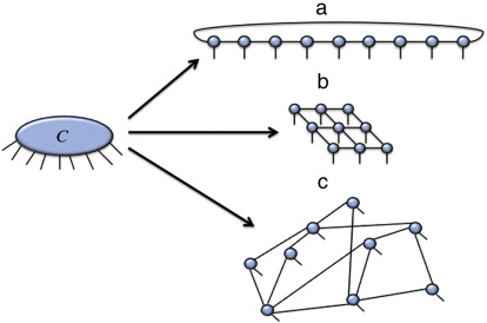
\includegraphics[width=0.5\columnwidth]{figure/TN.png}
    \caption{}
    \label{fig:TN}
\end{figure}

The left graph is the representation without any structural information, i.e., the solution can be expressed as in equation \ref{eq:general tensor product solution}. The three graphs on the right are representing three different structures of the tensor product space. For example, the structure in figure \ref{fig:TN}a represent periodic matrix product state, and the solution can be expressed in the way that
\begin{equation}\label{eq:MPS TN}
    A_{p_0,p_1,\cdots,p_{K-1}} = a^{(0)}_{b_{0},p_0,b_{1}}a^{(1)}_{b_{1},p_1,b_{2}}\cdots a^{(K-1)}_{b_{K-1},p_{K-1},b_{0}}
\end{equation}
where we assume Einstein's summation convention for any repreated indices. We can see that, if the maximum correlation degree, the number of values $b_k$'s in equation \ref{eq:MPS TN} can take, is $B_k$, the the total degree of freedom of the solution with this structure is
\begin{equation}
    \sum_{k=0}^{K-1}P_k\cdot B_k \cdot B_{k+1}
\end{equation}
with $B_K=B_0$. In other words, this structural information imposition to the problem can reduce the problem's complexity from exponential to polynomial.

\section{Target Equation}
In this work, we are considering a class of PDE that is linear in time (LT-PDE), as shown in equation \ref{eq:General LT-PDE}, of a tensor-valued function, $\tilde{\mathbf{u}}(t, \mathbf{q})$, of time, $t\in \mathbb{R}$, and $D$-dimensional space, $\mathbf{q}\in\mathbb{R}^D$, where we use boldface variables to indicate tensors:
\begin{equation}\label{eq:General LT-PDE}
    \tilde{\mathbf{h}}(t, \mathbf{q}, \tilde{\mathbf{u}}, \mathbf{D}_\mathbf{q}\tilde{\mathbf{u}}, \mathbf{D}_\mathbf{q}^2\tilde{\mathbf{u}}, \cdots) + \tilde{\mathbf{g}}_{1}(t, \mathbf{q})\text{D}_t\tilde{\mathbf{u}} + \tilde{\mathbf{g}}_{2}(t, \mathbf{q})\text{D}_t^2\tilde{\mathbf{u}} + \cdots = 0.
\end{equation}
Here, $\text{D}_t$ is time derivative operator, $\mathbf{D}_\mathbf{q}$ is spatial derivative tensor operator, $\tilde{\mathbf{h}}(\cdot)$ and $\tilde{\mathbf{g}}(\cdot)$'s are some functions, and the multiplication (and powers) between two tensors is their tensor product. Also, let the LT-PDE subjects to initial value 
\begin{equation}
    \tilde{\mathbf{u}}(t_0, \mathbf{q}) = \tilde{\mathbf{u}}^{(0)}(\mathbf{q}).
\end{equation}

It is common to treat a high-order linear ordinary differential equation (ODE) as multiple coupled first-order ODEs. We will apply the similar idea to the time derivative parts of our LT-PDE. Let's define the $\tau$-order time derivative of $\tilde{\mathbf{u}}$ as $\mathbf{u}_\tau$. Without loss of generality, let the LT-PDE has maximum time derivative order of $T$. Hence, equation \ref{eq:General LT-PDE} can be rewritten as
\begin{equation}\label{eq:Coupled LT-PDE}
    \left(
        \text{D}_t + 
        \begin{bmatrix}
            0 &-1 & 0 & \cdots & 0 \\
            0 & 0 &-1 & \cdots & 0 \\
            0 & 0 & 0 & \cdots & 0 \\
            \vdots & \vdots & \vdots & & \vdots \\
            0 & \dfrac{\tilde{\mathbf{g}}_1}{\tilde{\mathbf{g}}_{T}} & \dfrac{\tilde{\mathbf{g}}_2}{\tilde{\mathbf{g}}_{T}} & \cdots & \dfrac{\tilde{\mathbf{g}}_{T-1}}{\tilde{\mathbf{g}}_{T}} 
        \end{bmatrix}
    \right)
    \begin{bmatrix}
        \mathbf{u}_0 \\ \mathbf{u}_1 \\ \mathbf{u}_2 \\ \vdots \\ \mathbf{u}_{T-1}
    \end{bmatrix} +
    \begin{bmatrix}
        0 \\ 0 \\ 0 \\ \vdots \\ \dfrac{\tilde{\mathbf{h}}(t, \mathbf{q}, \mathbf{u}_0, \mathbf{D}_\mathbf{q}\mathbf{u}_0, \mathbf{D}_\mathbf{q}^2\mathbf{u}_0, \cdots)}{\tilde{\mathbf{g}}_{T}}
    \end{bmatrix} = 0.
\end{equation}
This means that, if we define $\mathbf{u}(t,\mathbf{q})$ as the tensor of $\mathbf{u}_\tau$'s, and $\mathbf{h}(t, \mathbf{q}, \mathbf{u}, \mathbf{D}_\mathbf{q}\mathbf{u}, \mathbf{D}_\mathbf{q}^2\mathbf{u}, \cdots)$ as the terms in equation \ref{eq:Coupled LT-PDE} that do not contain $\text{D}_t$, then the equation can be simplified to
\begin{equation}\label{eq:LT-PDE}
    \text{D}_t\mathbf{u} + \mathbf{h}(t, \mathbf{q}, \mathbf{u}, \mathbf{D}_\mathbf{q}\mathbf{u}, \mathbf{D}_\mathbf{q}^2\mathbf{u}, \cdots) = 0.
\end{equation}
Hence, we will assume, for the rest of the work that the LT-PDE contains only the first time derivative. We will also further restrict the tensor-valued function $\mathbf{h}(\cdot)$ to be analytic (ALT-PDE), i.e., it can be represented as a converging series:
\begin{equation}\label{eq:Analytic Function}
    \mathbf{h}(t, \mathbf{q}, \mathbf{u}, \mathbf{D}_\mathbf{q}\mathbf{u}, \mathbf{D}_\mathbf{q}^2\mathbf{u}, \cdots) = \sum_{i_0, i_1, i_2, \cdots\in\mathbb{Z}_{0+}} \left(\mathbf{h}_{i_0, i_1, i_2, \cdots}(t,\mathbf{q})\prod_{\chi\in\mathbb{Z}_{0+}}\left(\mathbf{D}_\mathbf{q}^\chi\mathbf{u}\right)^{i_\chi}\right),
\end{equation}
subjected to initial tensor-valued function
\begin{equation}\label{eq:Initial Function}
    \mathbf{u}(t_0, \mathbf{q}) = \mathbf{u}^{(0)}(\mathbf{q}).
\end{equation}

To set up for numerical calculation, we will discretize time for this section while the space discretization will be handle in the next section. Since the ALT-PDE is already framed in the context of initial value problem. We will adopt the common method where we will treat the time evolution part with FDM. Let's discretize equation \ref{eq:LT-PDE} into times $\{t_n|n\in\mathbb{Z}_{0+}\}$ with the function $\mathbf{u}$ defined at each time as
\begin{equation}\label{eq:Discretized Function}
    \mathbf{u}^{(n)}(\mathbf{q}) = \mathbf{u}(t_n, \mathbf{q}).
\end{equation} 
Also, define time steps as $\{\Delta_n=t_n-t_{n-1}|n\in\mathbb{Z}_{+}\}$. Here, we will use the first order method, i.e., Euler method, but it can be easily generalized to the higher one, e.g., Crank-Nicolson (second order), Runge-Kutta (forth order) methods, etc. With Euler method, equation \ref{eq:LT-PDE} can be written as two possible schemes:
\begin{equation}\label{eq:Explicit Euler}
    \mathbf{u}^{(n+1)} - \mathbf{u}^{(n)} + \Delta_{n+1}\mathbf{h}(t_{n}, \mathbf{q}, \mathbf{u}^{(n)}, \mathbf{D}_\mathbf{q}\mathbf{u}^{(n)}, \cdots) = 0,
\end{equation}
and
\begin{equation}\label{eq:Implicit Euler}
    \mathbf{u}^{(n+1)} - \mathbf{u}^{(n)} + \Delta_{n+1}\mathbf{h}(t_{n+1}, \mathbf{q}, \mathbf{u}^{(n+1)}, \mathbf{D}_\mathbf{q}\mathbf{u}^{(n+1)}, \cdots) = 0,
\end{equation}
where we implicitly omit the spatial dependence of $\mathbf{u}$ for neatness. These two are called explicit, and implicit time evolution schemes, respectively. While both of them are equivalent at the limit $\Delta\rightarrow0$, the first scheme can be unstable, and gives divergence if the number of time steps, or step sizes used are too large. Hence, for the remaining parts of this work we will only consider the implicit scheme method, i.e., equation \ref{eq:Implicit Euler}. In other words, we are solving ALT-PDE, for the time evolution part, with induction method from the initial value given by equation \ref{eq:Initial Function} such that, given the solution at time $t_n$, $\mathbf{u}^{(n)}$, we solve for solution at time $t_{n+1}$, $\mathbf{u}^{(n+1)}$, by tuning the function until it satisfies equation \ref{eq:Implicit Euler}. However, to make sure that such tuning is possible, we will modify the target equation into a convex optimization problem by introducing the least square error (LSE), 
\begin{equation}\label{eq:LSE}
    \text{LSE}_{n+1}(\mathbf{u}^{(n+1)}) = \int \left|\mathbf{u}^{(n+1)} - \mathbf{u}^{(n)} + \Delta_{n+1}\mathbf{h}(t_{n+1}, \mathbf{q}, \mathbf{u}^{(n+1)}, \mathbf{D}_\mathbf{q}\mathbf{u}^{(n+1)}, \cdots)\right|^2 d^D\mathbf{q}
\end{equation}
as the optimization target.

\section{Fourier Elemental Basis Representation}
From the previous section, in order to solve the ALT-PDE at each time step, one need to do convex optimization of the target function given by equation \ref{eq:LSE}. We will apply the FEM introduced before as the main method to do the optimization. In this section, we are going to introduce fourier basis representation for each element in FEM. For simplicity, from this section onward, we will only consider the case for one dimensional problem of a scalar-valued function, i.e., the target function can be simplified to
\begin{equation}\label{eq:1D scalar LSE}
    \text{LSE}_{n+1}(u^{(n+1)}) = \int \left|u^{(n+1)} - u^{(n)} + \Delta_{n+1}h(t_{n+1}, x, u^{(n+1)}, \partial_xu^{(n+1)}, \cdots)\right|^2 dx.
\end{equation}

With normal FEM, let's discretize the space into $K$ elements. Each element $k\in\{0, 1, \cdots, K-1\}$ has local coordinate centered at $x_k$, fundamental wavelength $\delta_k$, maximum fourier order $P_k$, and element's domain $\Omega_k=[x_{k,L}, x_{k, R}]$. Define the fourier basis for this element as
\begin{equation}
    S_k = \Set{\phi_{k,p_k\in[-P_k, P_k]}|\phi_{k,p_k}(x_k+x)=
                \begin{cases}
                    0 &; x_k + x \notin \Omega_k \\
                    1 &; p_k = 0\\
                    \sin(\dfrac{\pi p_k (x)}{\delta_k}) &; p_k > 0\\
                    \cos(\dfrac{\pi p_k (x)}{\delta_k}) &; p_k < 0
                \end{cases}
    }.
\end{equation}
There are many benefit of using Fourier basis. First, it is straight forward to calculate (approximate) derivatives, and functional multiplications in this representation. This means that, as long as $h$ is analytic, we can represent every term in equation \ref{eq:1D scalar LSE} as tensor equation. For the derivatives, we can directly use derivative of sine, and cosine functions as
\begin{equation}
    \partial_x\phi_{k,p_k} = \dfrac{\pi |p_k|}{\delta_k}
                                \begin{cases}
                                    0 &; p_k = 0 \\
                                    \phi_{k,-p_k} &; p_k > 0 \\
                                   -\phi_{k,-p_k} &; p_k < 0
                                \end{cases}.
\end{equation}
One can directly see that, the effect of derivatives can be captured by a matrix multiplication to a vector representation in this elemental basis. Let such matrix be $\mathbf{D}_k$ which, for any $\mathbf{v}$ in this subspace representation,
\begin{equation}
    [\partial_x^\chi \mathbf{v}]_i = [\mathbf{D}^\chi_{k}]_{i,j}v_j=D^\chi_{i, j}v_j
\end{equation}
where the last equality abuses notations for the compactness of formular. On the other hand, for functional multiplication, we can also use trigonometric identities as
\begin{equation}
    \phi_{k,p_{k,1}}\phi_{k,p_{k,2}} = \dfrac{1}{2}
        \begin{cases}
            -\phi_{k,p_{k,+}} + \phi_{k,p_{k,-}}  &; p_{k_1} > 0, p_{k_2} > 0 \\
            \phi_{k,-p_{k,+}} - \phi_{k,-p_{k,-}} &; p_{k_1} < 0, p_{k_2} > 0 \\
            \phi_{k,p_{k,+}} + \phi_{k,p_{k,-}}   &; \text{else}
        \end{cases}
\end{equation}
where $p_{k,+}=|p_{k, 1}|+|p_{k_2}|$, and $p_{k,-}=|p_{k, 1}|-|p_{k_2}|$. However, there are cases where $p_{k,+}>P_k$ which cannot be represented in our choice of basis. In those cases, we can simply cut out the terms to stay with in our basis. Because of this term truncation, one can also see that, the effect of functional multiplication can be captured by a tensor product decomposition between two vector representation in this elemental basis. Let the tensor corresponding to this be $\mathbf{R}_k$ which, for any $\mathbf{v}$, and $\mathbf{w}$ in this subspace representation,
\begin{equation}
    [\mathbf{v}\mathbf{w}]_i = [\mathbf{R}_{k}]_{i,j,k}v_jw_k=R_{i,j,k}v_jw_k
\end{equation}
where the last equality abuses notations for the compactness of formular.

The second benefit of this basis choice inherits from Fourier decomposition that the elemental basis functions are orthogonal which make it very convenient to calculate the functional square integration to be proportional to the Euclidean norm square of the representation, i.e., for any function $f$ represented by $\mathbf{v}$ in this subspace representation,
\begin{equation}
    \int_\Omega|f(x)|^2 dx \propto |\mathbf{v}|^2.
\end{equation}

The final benefit of this basis choice is that, as will be shown in the subsequent sections, with some reshaping, each optimization problem can be written with a close form of small rank matrix inversions, and multiplications similar to the result of multidimensional least square fitting when the PDE is also spatially linear.

\section{Tensor Optimization}
With the entangled basis representation introduced in the previous section, we are now applying such concept to the optimization of our target function, equation \ref{eq:1D scalar LSE}. First, we notice that the target function is in the form of the whole domain, i.e., the representation is with basis set $S=\cup_k S_k$. Since we can consider each element as its corresponding subspace that got tensor product to the whole domain, we can use the derivative matrices, and functional multiplicative tensors of each element to construct the whole space version as
\begin{equation}
    D_{\alpha,\beta} = D_{\alpha_0,\beta_0}D_{\alpha_1,\beta_1}\cdots D_{\alpha_{K-1},\beta_{K-1}},
\end{equation}
and
\begin{equation}
    R_{\alpha,\beta,\gamma} = R_{\alpha_0,\beta_0,\gamma_0}R_{\alpha_1,\beta_1,\gamma_1}\cdots R_{\alpha_{K-1},\beta_{K-1},\gamma_{K-1}}.
\end{equation}

From these, we can rewrite equation \ref{eq:1D scalar LSE} with our representation as
\begin{equation}
    \left|U^{(n+1)}_\alpha - U^{(n)}_\alpha + \Delta_{n+1}\sum_{i_0, i_1, i_2, \cdots\in\mathbb{Z}_{0+}} R^{\sum_\chi i_\chi}\left(H^{(n+1)}_{i_0, i_1, i_2, \cdots}\prod_{\chi\in\mathbb{Z}_{0+}}\left(D^\chi U^{(n+1)}\right)^{i_\chi}\right)\right|^2
\end{equation}
where $U$'s, and $H$'s are $u$'s, and $h$'s representation in our basis $S$, and we abuse the notation by omitting the matrices, and tensors' indices for the last term. We can see that we successfully transform our original PDE problem, into a tensorial convex optimization problem which campatible to quantum computation qubit set up, and enable the possibility of utilizing quantum computer as the plat form for PDE solver.

For the remaining parts of this work, we will limit the class of problem down to linear PDE, i.e., spatially linear as well. In this case, the target function further simplifies to
\begin{equation}
    \left|U^{(n+1)}_\alpha - U^{(n)}_\alpha + \Delta_{n+1}\sum_{\chi\in\mathbb{Z}_{0+}} R_{\alpha\gamma\eta}H^{(n+1)}_{\chi, \gamma}D^\chi_{\eta,\beta} U^{(n+1)}_\beta\right|^2.
\end{equation}
We can rearrange the terms to

\section{Matrix Product State (MPS) Representation}
To show some concrete example, in this section, we are going to specialize the problem for the case where we already got efficient way (algorithm) to do TN optimization. 

\begin{figure}[ht!]
    \centering
    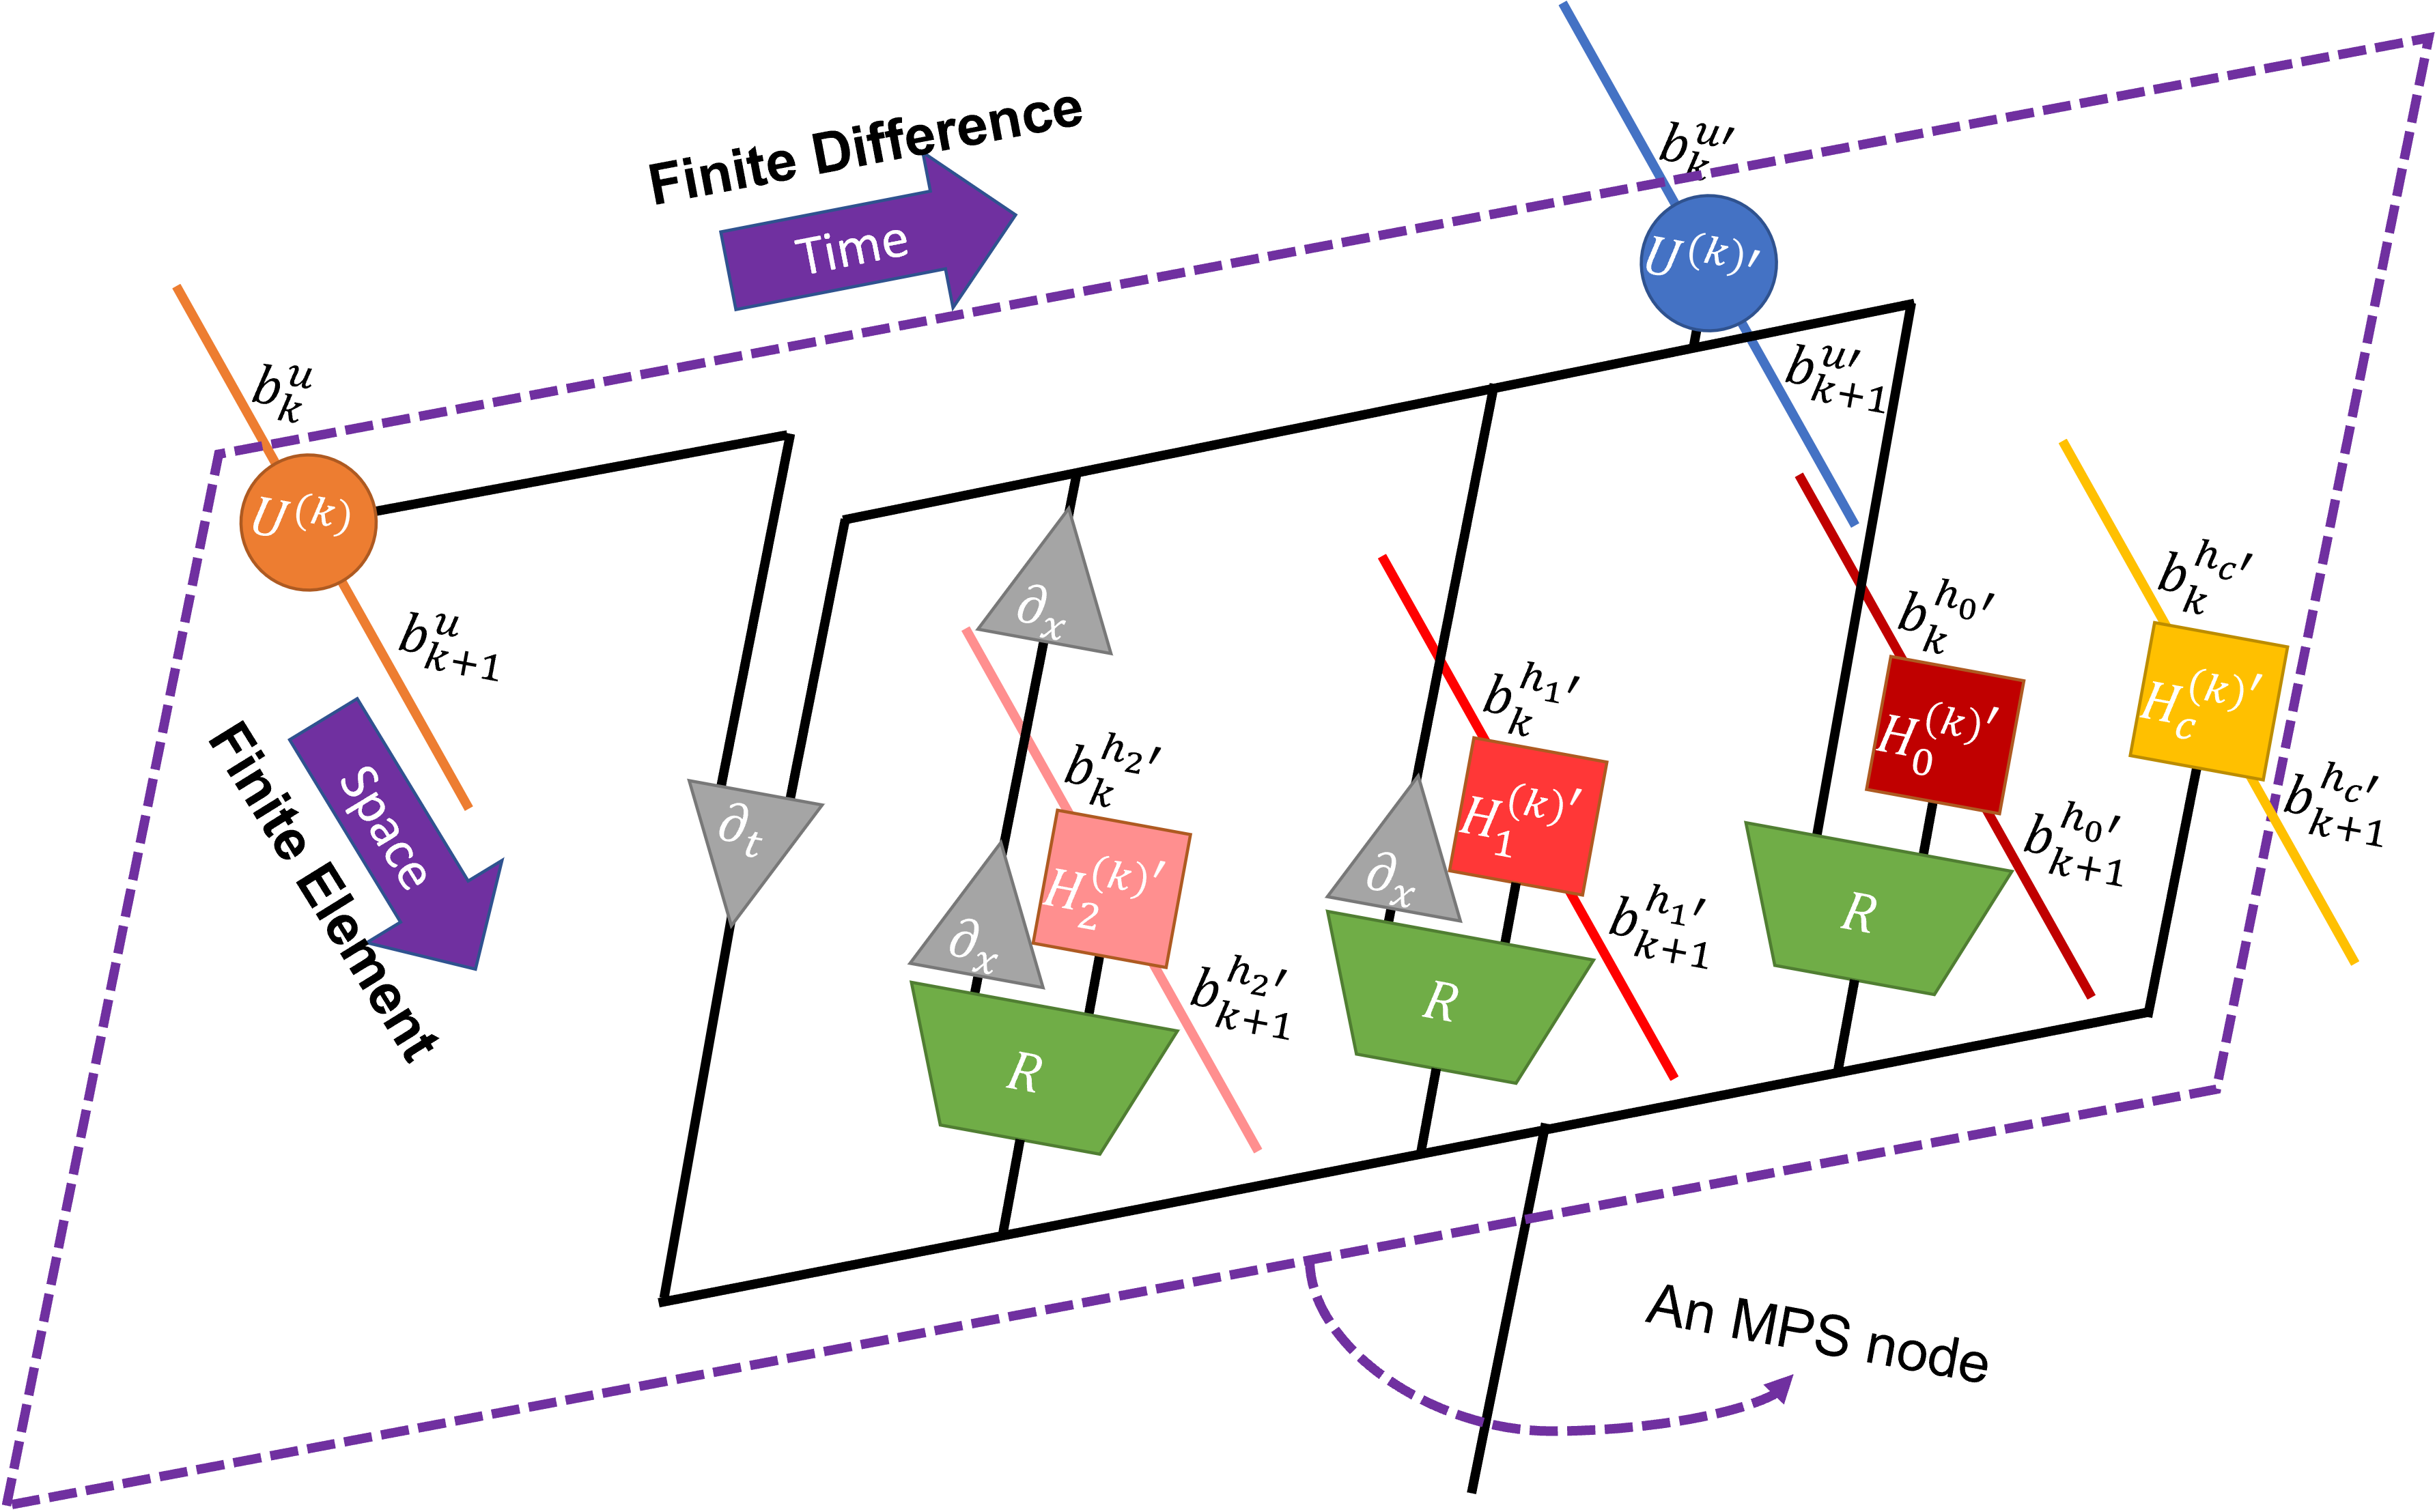
\includegraphics[width=0.8\columnwidth]{figure/MPS.png}
    \caption{}
    \label{fig:MPS}
\end{figure}

\section{Implementation}

\end{document}